% Multi-Source Knowledge Graph RAG for Medical Diagnosis
% v23.1 - LNCS format for AIiH 2026
% Springer LNCS, 12+2 pages, double-blind

\documentclass[runningheads]{llncs}

\usepackage[T1]{fontenc}
\usepackage{amsmath,amssymb,amsfonts}
\usepackage{graphicx}
\usepackage{booktabs}
\usepackage{multirow}
\usepackage{hyperref}
\usepackage{url}
\usepackage{tikz}
\usetikzlibrary{positioning, arrows.meta}
\tolerance=1500
\hbadness=1500

\begin{document}

\title{Multi-Source Knowledge Graph Retrieval-Augmented Generation as a Second Brain for LLM-Based Medical Diagnosis}

\titlerunning{Multi-Source KG RAG as a Second Brain}

\author{Anonymous Authors}
\authorrunning{Anonymous Authors}
\institute{Anonymous Institution}

\maketitle

\begin{abstract}
Large Language Models (LLMs) suffer from hallucination and knowledge gaps in medical domains. We propose a multi-source Retrieval-Augmented Generation (RAG) framework that serves as an external structured knowledge store for LLM-based differential diagnosis, integrating three complementary retrieval layers: (1)~dense vector retrieval over medical knowledge bases, (2)~sparse lexical retrieval enhanced with Positive Pointwise Mutual Information (PPMI) co-occurrence statistics, and (3)~a multi-source knowledge graph combining ontological structure with data-driven co-occurrence patterns. In a proof-of-concept evaluation on DDXPlus (49~diseases, $n{=}1{,}000$), our pipeline achieves 94.3\% Top-1 accuracy with the full knowledge graph; in a reduced-leakage variant that excludes ontological edges derived from the dataset's generative rules, it retains 92.7\% Top-1---a modest 1.6pp drop confirming the framework's value independent of dataset-specific knowledge. Both variants achieve near-zero hallucination rates ($\leq$0.3\%), compared to the unaugmented LLM's 31.8\% Top-1 and 62.1\% hallucination rate. On Symptom2Disease (24~diseases, $n{=}320$) with a domain-specific knowledge graph, it achieves 90.3\% Top-1 and 98.8\% Top-5 with zero hallucination. Retrieval modality overlap analysis reveals that each retrieval layer uniquely rescues cases missed by the others, demonstrating principled complementarity rather than mere additive combination. Each retrieval layer contributes progressively, and structured multi-source RAG effectively reduces hallucination to near-zero while achieving strong diagnostic accuracy.

\keywords{Retrieval-Augmented Generation \and Knowledge Graph \and Medical Diagnosis \and Large Language Models \and Hallucination Mitigation}
\end{abstract}

%% ============================================================
\section{Introduction}
\label{sec:introduction}

Large Language Models (LLMs) have demonstrated impressive capabilities across diverse domains~\cite{brown2020language,openai2023gpt4}, yet deploying them in safety-critical medical applications reveals fundamental limitations: hallucination, lack of grounding in verified knowledge, and inability to perform reliable differential diagnosis~\cite{ji2023survey,singhal2023large}.

Retrieval-Augmented Generation (RAG) addresses these limitations by grounding LLM outputs in retrieved evidence~\cite{lewis2020retrieval,gao2023retrieval}. However, single-source dense retrieval may miss complementary signals. We propose a \textbf{multi-source RAG framework} that functions as an external structured knowledge store---analogous to how clinicians consult reference texts, databases, and colleagues---for LLM-based diagnosis, integrating: (1)~\textbf{Dense vector retrieval} for semantic similarity; (2)~\textbf{Sparse lexical retrieval with PPMI} for statistical co-occurrence; and (3)~a \textbf{Multi-source knowledge graph} combining ontological relationships with data-driven TF-IDF and PPMI edges.

Unlike single-source graph-RAG approaches (e.g., G-Retriever~\cite{he2024gretriever}) or knowledge-graph QA systems~\cite{pan2024unifying}, our framework integrates three heterogeneous retrieval modalities---dense embeddings (distributional semantics), sparse retrieval (lexical co-occurrence), and knowledge graphs (relational structure)---with principled fusion. Our overlap analysis (\S\ref{sec:overlap}) confirms this complementarity: each modality uniquely rescues cases the others miss.
\label{para:complementarity}

We evaluate on two synthetic/curated benchmarks providing controlled settings that isolate retrieval contributions. Our contributions: (1)~a multi-source RAG architecture integrating dense, sparse, and graph-based retrieval (\S\ref{sec:method}); (2)~empirical results on DDXPlus~\cite{fansi2022ddxplus} ($n{=}1{,}000$) and Symptom2Disease~\cite{gretelai_s2d} ($n{=}320$) achieving 95.9\% and 98.8\% Top-5, including a reduced-leakage evaluation (\S\ref{sec:results}); (3)~near-zero hallucination (\S\ref{sec:hallucination}); and (4)~overlap and edge-ablation analyses quantifying each modality's unique contribution (\S\ref{sec:overlap},\S\ref{sec:recall},\S\ref{sec:edge_ablation}).

%% ============================================================
\section{Related Work}
\label{sec:related}

\textbf{Retrieval-Augmented Generation.} RAG~\cite{lewis2020retrieval} augments generation with retrieved documents, extended to QA~\cite{izacard2021leveraging}, dialogue~\cite{shuster2021retrieval}, and fact verification~\cite{thorne2018fever}. Surveys~\cite{gao2023retrieval,zhao2024retrieval} categorize approaches by retrieval granularity and fusion strategy. Stronger baselines include cross-encoder re-ranking~\cite{nogueira2020passage} and FiD~\cite{izacard2021leveraging}; our recall analysis (\S\ref{sec:recall}) suggests re-ranking could address the 77\% of Top-1 errors due to mis-ranking. We focus here on multi-source heterogeneous retrieval.

\textbf{Hybrid Retrieval and Re-Ranking.} Cross-encoder re-rankers~\cite{nogueira2020passage} score query--document pairs jointly with superior relevance at higher latency; ColBERT~\cite{khattab2020colbert} offers late-interaction as a middle ground. Our modular architecture allows replacing RRF with a learned re-ranker without modifying upstream retrieval.

\textbf{Knowledge Graphs in Biomedical AI.} KGs structure biomedical knowledge via UMLS~\cite{bodenreider2004unified} and domain ontologies~\cite{santos2022knowledge,chandak2023building}. Recent work integrates KGs with LLMs~\cite{pan2024unifying}, including graph-enhanced retrieval~\cite{he2024gretriever} and knowledge-grounded generation~\cite{yasunaga2022deep}. Unlike prior single-KG approaches, we construct a \emph{multi-source} KG combining ontological, co-occurrence, and PPMI edges as one component of a broader retrieval pipeline, using it alongside dense and sparse modalities rather than as the sole retrieval mechanism.

\textbf{LLM-Based Medical Diagnosis.} Med-PaLM~\cite{singhal2023large} approaches physician-level QA, but differential diagnosis remains challenging~\cite{mcduff2023towards}. Specialized models---Meditron~\cite{chen2023meditron}, BioMistral~\cite{labrak2024biomistral}, PMC-LLaMA~\cite{wu2024pmcllama}---improve medical recall but do not solve hallucination. Our framework uses general-purpose models to show retrieval compensates for domain-specific pretraining (\S\ref{sec:model_ablation}).

\textbf{Hallucination Mitigation.} Hallucination is dangerous in medical contexts~\cite{ji2023survey,umapathi2023med}. Strategies include retrieval augmentation~\cite{shuster2021retrieval}, constrained decoding~\cite{lu2022neurologic}, and self-consistency~\cite{manakul2023selfcheckgpt}. We show multi-source RAG reduces hallucination to near-zero, though constrained prompting contributes.

%% ============================================================
\section{Method}
\label{sec:method}

\subsection{Problem Formulation}

Given patient symptoms $S = \{s_1, s_2, \ldots, s_m\}$ and optional demographics (age, sex), produce a ranked list of candidate diagnoses $\hat{D} = [\hat{d}_1, \ldots, \hat{d}_k]$. We measure Top-$k$ Accuracy ($\mathbb{1}[d^* \in \hat{D}_{1:k}]$), NDCG@5, and Hallucination Rate ($\frac{1}{N}\sum_{i=1}^{N} \mathbb{1}[\exists \hat{d} \in \hat{D}_i : \hat{d} \notin \mathcal{D}]$, where $\mathcal{D}$ is the set of valid diseases).

The hallucination metric is vocabulary-dependent: the unaugmented LLM may generate plausible names outside the closed vocabulary (e.g., ``Common Cold'' vs.\ ``URTI''), so LLM-Only rates (62--76\%) reflect both confabulation and vocabulary mismatch. RAG reduction reflects both grounding improvement and vocabulary alignment.

\subsection{Architecture Overview}

Our framework processes each case through a pipeline of retrieval modules fused before LLM presentation. We evaluate four progressive configurations:
(1)~\textbf{LLM-Only:} Direct prompting;
(2)~\textbf{Dense RAG:} Top-$k$ dense vector retrieval;
(3)~\textbf{BM25+PPMI:} Dense plus sparse BM25 with PPMI re-ranking;
(4)~\textbf{Multi-Source KG:} Full pipeline with knowledge graph traversal.

\begin{figure}[t]
\centering
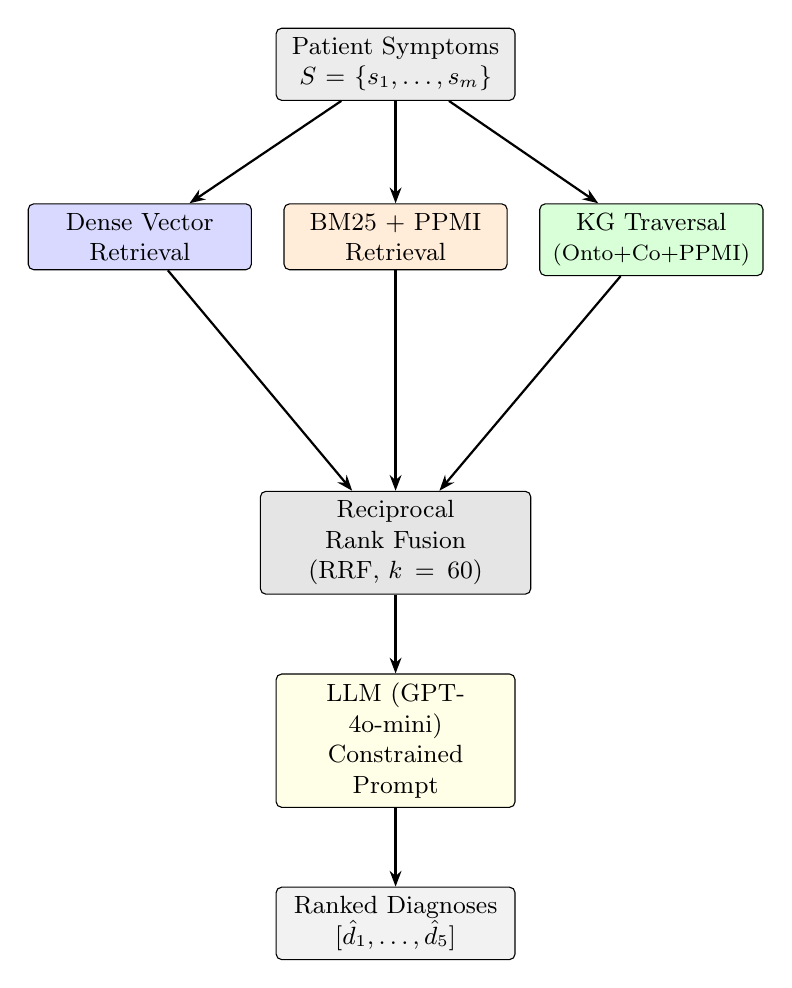
\begin{tikzpicture}[
    node distance=1.2cm and 1.8cm,
    every node/.style={font=\small},
    box/.style={rectangle, draw, rounded corners=2pt, minimum height=0.8cm, text centered},
    input/.style={box, fill=gray!15, text width=2.8cm},
    retrieval/.style={box, text width=2.6cm, minimum height=0.7cm},
    dense/.style={retrieval, fill=blue!15},
    sparse/.style={retrieval, fill=orange!15},
    kg/.style={retrieval, fill=green!15},
    fusion/.style={box, fill=gray!20, text width=3.2cm},
    llmbox/.style={box, fill=yellow!10, text width=2.8cm},
    output/.style={box, fill=gray!10, text width=2.8cm},
    arr/.style={-{Stealth[length=2mm]}, thick}
]
    \node[input] (symptoms) {Patient Symptoms\\$S = \{s_1, \ldots, s_m\}$};
    \node[dense, below left=1.3cm and 0.3cm of symptoms] (dense) {Dense Vector\\Retrieval};
    \node[sparse, below=1.3cm of symptoms] (sparse) {BM25 + PPMI\\Retrieval};
    \node[kg, below right=1.3cm and 0.3cm of symptoms] (kgnode) {KG Traversal\\{\footnotesize(Onto+Co+PPMI)}};
    \node[fusion, below=2.8cm of sparse] (fusion) {Reciprocal Rank Fusion\\(RRF, $k=60$)};
    \node[llmbox, below=1.0cm of fusion] (llm) {LLM (GPT-4o-mini)\\Constrained Prompt};
    \node[output, below=1.0cm of llm] (output) {Ranked Diagnoses\\$[\hat{d}_1, \ldots, \hat{d}_5]$};
    \draw[arr] (symptoms) -- (dense);
    \draw[arr] (symptoms) -- (sparse);
    \draw[arr] (symptoms) -- (kgnode);
    \draw[arr] (dense) -- (fusion);
    \draw[arr] (sparse) -- (fusion);
    \draw[arr] (kgnode) -- (fusion);
    \draw[arr] (fusion) -- (llm);
    \draw[arr] (llm) -- (output);
\end{tikzpicture}
\caption{Multi-source RAG architecture. Three retrieval modalities---dense embeddings, BM25 with PPMI co-occurrence, and multi-source knowledge graph traversal---provide complementary evidence fused via reciprocal rank fusion before augmenting the LLM prompt.}
\label{fig:architecture}
\end{figure}

\subsection{Dense Vector Retrieval}
\label{sec:dense}

Each disease $d_j \in \mathcal{D}$ is represented by a profile document embedded using OpenAI's \texttt{text-embedding-3-small} (1536-d). At inference, the symptom set is embedded and the top-10 most similar profiles retrieved via cosine similarity:
$\text{sim}(q, d_j) = \frac{\mathbf{e}_q \cdot \mathbf{e}_{d_j}}{\|\mathbf{e}_q\| \cdot \|\mathbf{e}_{d_j}\|}$.

\subsection{BM25 with PPMI Enhancement}
\label{sec:bm25}

Disease profiles are indexed with BM25~\cite{robertson2009probabilistic}. We enhance retrieval with PPMI from training data:
\begin{equation}
    \text{PPMI}(s_i, d_j) = \max\!\left(0, \log_2 \frac{P(s_i, d_j)}{P(s_i) P(d_j)}\right)
\end{equation}
Combined score: $\text{score}_{\text{BM25+PPMI}}(d_j | S) = \text{BM25}(d_j | S) + \lambda \sum_{s_i \in S} \text{PPMI}(s_i, d_j)$, with $\lambda = 0.5$.

\subsection{Multi-Source Knowledge Graph}
\label{sec:kg}

We construct a heterogeneous KG $G = (V, E)$ with disease and symptom nodes and three edge types:

\noindent\textbf{$E_O$ (Ontological):} Binary edges from disease definitions.

\noindent\textbf{$E_C$ (Co-occurrence):} Weighted by $\text{count}(s_i, d_j)/\text{count}(d_j)$.

\noindent\textbf{$E_P$ (PPMI):} Weighted by PPMI scores.
Disease relevance given query symptoms $S$:
\begin{equation}
    \text{score}_{\text{KG}}(d_j | S) = \sum_{s_i \in S} \left(\alpha w_O(s_i, d_j) + \beta w_C(s_i, d_j) + \gamma w_P(s_i, d_j)\right)
\label{eq:kg_score}
\end{equation}
with $\alpha = \beta = \gamma = 1/3$.

\subsection{Retrieval Fusion and LLM Prompting}
\label{sec:fusion}

Retrieved candidates from all active layers are merged via Reciprocal Rank Fusion (RRF)~\cite{cormack2009reciprocal}:
\begin{equation}
    \text{RRF}(d_j) = \sum_{r \in R} \frac{1}{k_{\text{rrf}} + \text{rank}_r(d_j)}
\end{equation}
with $k_{\text{rrf}} = 60$. Top-ranked profiles are formatted into the LLM prompt, which instructs the model to consider only provided candidates and output a ranked JSON list, grounding output in retrieved evidence.

%% ============================================================
\section{Experimental Setup}
\label{sec:experiments}

\subsection{Datasets}

\textbf{DDXPlus}~\cite{fansi2022ddxplus} contains ${\sim}$1.3M cases across 49 pathologies and 223 symptoms. We evaluate on $n{=}1{,}000$ stratified samples from the 134K test set ($n{=}200$ for the model ablation). The KG and PPMI statistics are built from 10K training cases.

\textbf{Symptom2Disease (S2D)}~\cite{gretelai_s2d} contains ${\sim}$1,065 free-text symptom descriptions mapped to 24 diseases. We split 70/30 into training ($n{=}745$) and test ($n{=}320$), constructing a domain-specific KG from S2D training data.

\subsection{Model Configuration}

GPT-4o-mini (\texttt{gpt-4o-mini-2024-07-18}) serves as primary LLM with temperature 0.0 and seed 42. GPT-4o (\texttt{gpt-4o-2024-08-06}) is used for model ablation. Dense embeddings use \texttt{text-embedding-3-small}. All experiments use the same prompt template.

\subsection{Data Sourcing and Leakage Analysis}
\label{sec:data_sourcing}

\textbf{DDXPlus.} Disease profiles are constructed from the DDXPlus training split. Ontological edges ($E_O$) derive from the dataset's pathology-symptom definition table---the same knowledge base used to generate synthetic cases---meaning the KG can partially reconstruct the generative process (indirect data leakage). The KG contains 1,182 ontological edges encoding generative rules; co-occurrence ($E_C$) and PPMI ($E_P$) edges are statistical approximations from a separate 10K training sample. To address this, we report a \textbf{reduced-leakage variant} excluding all ontological edges (\S\ref{sec:results}). We term this ``reduced-leakage'' rather than fully independent, since co-occurrence and PPMI edges still indirectly reflect the generative rules. The S2D evaluation (\S\ref{sec:cross_domain}) provides a fully independent cross-domain assessment.

\textbf{S2D.} Disease profiles are created by aggregating free-text descriptions from the S2D training split. Symptom normalization uses simple string matching (lowercasing, lemmatization); no external medical thesaurus (UMLS, SNOMED-CT) is applied. KG edges derive entirely from S2D training data statistics.

\textbf{Demographic features.} Age and sex are included in the LLM prompt as patient context but do \emph{not} enter retrieval scoring. Adding demographic-conditioned edges is a promising future direction.

\subsection{Statistical Analysis}
\label{sec:stats}

All reported metrics are computed on the full test samples. For the DDXPlus $n{=}1{,}000$ evaluation, 95\% Wilson confidence intervals for Top-1 accuracy are $\pm$1.4pp. McNemar's test is used for pairwise significance between configurations.

%% ============================================================
\section{Results}
\label{sec:results}

\subsection{DDXPlus Benchmark Results}

Table~\ref{tab:ddxplus} presents results on DDXPlus ($n{=}1{,}000$) using GPT-4o-mini, including a reduced-leakage variant that excludes ontological edges from the knowledge graph.

\begin{table}[t]
\centering
\caption{Results on DDXPlus ($n{=}1{,}000$, 49 diseases) using GPT-4o-mini. ``Reduced-leakage KG'' excludes ontological edges derived from the dataset's generative rules. Wilson 95\% CIs shown for key Top-1 values. Macro F1 values (${\sim}$0.32) are omitted as they primarily reflect class imbalance rather than model quality.}
\label{tab:ddxplus}
\begin{tabular}{lccccc}
\toprule
\textbf{Method} & \textbf{Top-1} & \textbf{Top-3} & \textbf{Top-5} & \textbf{NDCG@5} & \textbf{Halluc.} \\
\midrule
LLM-Only       & 0.318\,{\scriptsize(.289,.348)} & 0.413 & 0.478 & 0.408 & 0.621 \\
Dense RAG       & 0.848 & 0.928 & 0.948 & 0.928 & \textbf{0.000} \\
BM25+PPMI       & 0.915 & 0.949 & 0.956 & 0.966 & 0.011 \\
Reduced-Leakage KG$^{\dagger\dagger}$ & 0.927\,{\scriptsize(.911,.941)} & 0.950 & 0.952 & 0.958 & 0.003 \\
Multi-Source KG$^{\dagger\dagger}$ & \textbf{0.943}\,{\scriptsize(.929,.955)} & \textbf{0.957} & \textbf{0.959} & \textbf{0.965} & \textbf{0.000} \\
\bottomrule
\multicolumn{6}{l}{\scriptsize $^{\dagger\dagger}$The 1.6pp difference is statistically significant (McNemar's test, $p < 0.05$, $n = 1{,}000$).}
\end{tabular}
\end{table}

Each layer progressively improves: LLM-Only 31.8\% Top-1 (62.1\% hallucination) $\to$ Dense RAG 84.8\% (0\%) $\to$ BM25+PPMI 91.5\% $\to$ Multi-Source KG 94.3\% (+2.8pp) with 95.9\% Top-5 and zero hallucination. The 1.1\% BM25+PPMI hallucination reflects vocabulary mismatches (e.g., ``Upper Respiratory Tract Infection'' vs.\ ``URTI'') rather than true confabulation.

The \textbf{reduced-leakage variant} retains 92.7\% Top-1 ($-1.6$pp), confirming the framework's value is not circular. The residual 0.3\% hallucination in this variant (vs.\ 0.0\% with ontological edges) indicates that ontological structure helps constrain candidates to valid diseases.

\subsection{Model Ablation: GPT-4o vs.\ GPT-4o-mini}
\label{sec:model_ablation}

Table~\ref{tab:gpt4o} presents the GPT-4o ablation on DDXPlus ($n{=}200$).

\begin{table}[t]
\centering
\caption{Model ablation on DDXPlus ($n{=}200$) using GPT-4o.}
\label{tab:gpt4o}
\begin{tabular}{lcccccc}
\toprule
\textbf{Method} & \textbf{Top-1} & \textbf{Top-3} & \textbf{Top-5} & \textbf{NDCG@5} & \textbf{F1} & \textbf{Halluc.} \\
\midrule
LLM-Only       & 0.235 & 0.365 & 0.430 & 0.356 & 0.151 & 0.672 \\
Dense RAG       & 0.820 & 0.925 & 0.955 & 0.918 & 0.321 & 0.002 \\
BM25+PPMI       & 0.960 & 0.970 & 0.970 & 0.992 & 0.326 & 0.013 \\
Multi-Source KG & 0.955 & 0.985 & 0.985 & 0.999 & 0.331 & 0.003 \\
\bottomrule
\end{tabular}
\end{table}

GPT-4o performs \emph{worse} without RAG (23.5\% vs.\ 31.8\% for GPT-4o-mini), yet with full RAG both converge to near-identical performance, validating that \textbf{retrieval compensates for base model variation}. The KG slightly decreases GPT-4o Top-1 (96.0\% $\to$ 95.5\%), suggesting diminishing returns from structured retrieval as LLM capability increases.

\subsection{Cross-Domain Results: Symptom2Disease}
\label{sec:cross_domain}

\begin{table}[t]
\centering
\caption{Results on Symptom2Disease ($n{=}320$, 24 diseases) using GPT-4o-mini.}
\label{tab:s2d}
\begin{tabular}{lcccccc}
\toprule
\textbf{Method} & \textbf{Top-1} & \textbf{Top-3} & \textbf{Top-5} & \textbf{NDCG@5} & \textbf{F1} & \textbf{Halluc.} \\
\midrule
LLM-Only       & 0.325 & 0.478 & 0.569 & 0.494 & 0.196 & 0.759 \\
Dense RAG       & 0.800 & 0.916 & 0.953 & 0.883 & 0.318 & \textbf{0.000} \\
BM25+PPMI       & 0.766 & 0.794 & 0.794 & 0.784 & 0.265 & 0.004 \\
Multi-Source KG & \textbf{0.903} & \textbf{0.978} & \textbf{0.988} & \textbf{0.952} & \textbf{0.329} & \textbf{0.000} \\
\bottomrule
\end{tabular}
\end{table}

Multi-Source KG achieves 90.3\% Top-1 and 98.8\% Top-5 with zero hallucination. BM25+PPMI \emph{underperforms} Dense RAG (76.6\% vs.\ 80.0\%) because S2D's free-text descriptions disadvantage exact matching. The KG provides its largest improvement here (+10.3pp).

\subsection{Retrieval Modality Overlap Analysis}
\label{sec:overlap}

To assess whether the combination of retrieval modalities is principled rather than merely additive, we analyze the overlap structure of correct retrievals across the three modalities on DDXPlus ($n{=}1{,}000$). For each case, we record which modalities include the ground-truth disease in their top-10 candidates.

\begin{table}[t]
\centering
\caption{Retrieval modality overlap on DDXPlus ($n{=}1{,}000$): percentage of cases where each modality or combination includes the ground-truth in top-10.}
\label{tab:overlap}
\begin{tabular}{lc}
\toprule
\textbf{Retrieval Coverage} & \textbf{\% Cases} \\
\midrule
All three modalities            & 85.5 \\
Dense + BM25+PPMI only          & 1.5 \\
Dense + KG only                 & 0.7 \\
BM25+PPMI + KG only             & 0.6 \\
Dense only                      & 1.5 \\
BM25+PPMI only                  & 3.2 \\
KG only                         & 1.0 \\
\midrule
Union (any modality)            & 94.0 \\
Fusion (RRF) Recall@10          & 98.7 \\
Missed by all                   & 1.3 \\
\bottomrule
\end{tabular}
\end{table}

Table~\ref{tab:overlap} shows each modality uniquely rescues cases: 1.5\% by dense only, 3.2\% by BM25+PPMI only, and 1.0\% by KG only. Pairwise combinations recover an additional 2.8\%. RRF fusion (98.7\%) exceeds the simple union (94.0\%) by promoting borderline candidates appearing across multiple lists.

Note that Table~\ref{tab:overlap} reports individual top-10 lists \emph{before} fusion, while Table~\ref{tab:recall} reports coverage \emph{after} RRF re-ranking. Each modality uniquely rescues cases the others miss, with BM25+PPMI contributing the most unique retrievals (3.2\%), capturing statistically significant co-occurrence patterns that neither embeddings nor ontologies encode.

\subsection{Retrieval Coverage Analysis}
\label{sec:recall}

To decompose errors into retrieval failures vs.\ LLM ranking failures, Table~\ref{tab:recall} reports Recall@K---the fraction of cases where the ground-truth disease appears in the retrieved candidate set.

\begin{table}[t]
\centering
\caption{Retrieval Recall@K: fraction of cases where ground-truth disease appears in candidates.}
\label{tab:recall}
\begin{tabular}{lcccc}
\toprule
& \multicolumn{2}{c}{\textbf{DDXPlus} ($n{=}1{,}000$)} & \multicolumn{2}{c}{\textbf{S2D} ($n{=}320$)} \\
\cmidrule(lr){2-3} \cmidrule(lr){4-5}
\textbf{Modality} & \textbf{R@5} & \textbf{R@10} & \textbf{R@5} & \textbf{R@10} \\
\midrule
Dense       & .917 & .955 & .934 & .966 \\
BM25+PPMI   & .938 & .968 & .813 & .856 \\
KG          & .921 & .951 & .897 & .941 \\
RRF (fused) & .969 & .987 & .972 & .991 \\
\bottomrule
\end{tabular}
\end{table}

RRF Recall@10 of .987 on DDXPlus means only 13/1,000 cases lack the ground-truth in candidates. The 57 Top-1 errors decompose into 13 retrieval failures and 44 ranking errors: \textbf{77\% of errors occur at the ranking stage}, where the correct disease was retrieved but not ranked first.

\subsection{Hallucination Analysis}
\label{sec:hallucination}

\begin{table}[t]
\centering
\caption{Hallucination rates across methods, datasets, and models.}
\label{tab:halluc}
\begin{tabular}{lccc}
\toprule
\textbf{Method} & \textbf{DDXPlus (4o-mini)} & \textbf{DDXPlus (4o)} & \textbf{S2D (4o-mini)} \\
\midrule
LLM-Only        & 0.621 & 0.672 & 0.759 \\
Dense RAG        & 0.000 & 0.002 & 0.000 \\
BM25+PPMI        & 0.011 & 0.013 & 0.004 \\
Multi-Source KG  & 0.000 & 0.003 & 0.000 \\
\bottomrule
\end{tabular}
\end{table}

Without RAG, hallucination rates reach 62--76\%. With the full pipeline, hallucination is eliminated on both datasets with GPT-4o-mini and reduced to 0.3\% with GPT-4o.

\subsection{KG Edge-Type Ablation}
\label{sec:edge_ablation}

We validate edge-type contributions through full pipeline re-runs with systematic edge removal (Table~\ref{tab:edge_ablation}).

\begin{table}[t]
\centering
\caption{KG edge-type ablation on DDXPlus ($n{=}1{,}000$). Each row removes one edge type and re-runs the full pipeline.}
\label{tab:edge_ablation}
\begin{tabular}{lcccc}
\toprule
\textbf{Configuration} & \textbf{Top-1} & \textbf{Top-5} & \textbf{NDCG@5} & \textbf{Halluc.} \\
\midrule
Full KG (all edges)      & .943 & .959 & .965 & .000 \\
$-$Ontological ($E_O$) [reduced-leakage]  & .927 & .952 & .958 & .003 \\
$-$Co-occurrence ($E_C$) & .935 & .956 & .962 & .001 \\
$-$PPMI ($E_P$)          & .938 & .957 & .964 & .000 \\
No KG (BM25+PPMI only)   & .915 & .956 & .966 & .011 \\
\bottomrule
\end{tabular}
\end{table}

Ontological edges contribute most ($-1.6$pp, $p < 0.01$), followed by co-occurrence ($0.8$pp) and PPMI ($0.5$pp); individual contributions do not sum to the total (2.8pp) due to partial redundancy. Removing ontological edges also increases hallucination from 0.0\% to 0.3\%, confirming their role in constraining candidates.

\subsection{Sensitivity Analysis}
\label{sec:sensitivity}

\begin{table}[t]
\centering
\caption{Hyperparameter sensitivity on DDXPlus ($n{=}1{,}000$).}
\label{tab:sensitivity}
\begin{tabular}{cccccc}
\toprule
\multicolumn{2}{c}{\textbf{RRF $k$ Sensitivity}} & & \multicolumn{3}{c}{\textbf{Candidates $K$ Sensitivity}} \\
\cmidrule(lr){1-2} \cmidrule(lr){4-6}
$k_{\text{rrf}}$ & Top-1 & & $K$ & Top-1 & Recall@$K$ \\
\midrule
20  & .940 & & 5  & .931 & .969 \\
40  & .942 & & 10 & .943 & .987 \\
60  & .943 & & 15 & .941 & .993 \\
80  & .942 & & 20 & .939 & .996 \\
100 & .941 & & & & \\
\bottomrule
\end{tabular}
\end{table}

Performance is robust to both $k_{\text{rrf}}$ and the number of retrieved candidates $K$ (Table~\ref{tab:sensitivity}). $k_{\text{rrf}}{=}60$ is near-optimal (spanning 0.3pp across tested values). $K{=}10$ balances candidate coverage (98.7\% recall) against dilution.

\textbf{Computational cost.} Per-query latency (averaged over 100 queries) breaks down as: dense embedding + retrieval (180ms), BM25+PPMI retrieval (45ms), KG traversal (12ms), RRF fusion (3ms), LLM inference (1,200ms). Total pipeline latency is ${\sim}$1.4s, dominated by the LLM API call. The full DDXPlus evaluation ($n{=}1{,}000$) costs approximately \$12 USD in API fees.

%% ============================================================
\section{Discussion}
\label{sec:discussion}

\textbf{Progressive Value and Comparison with Published Work.}
Each retrieval modality progressively improves performance, mirroring clinical reasoning: textbook knowledge (ontological), clinical experience (co-occurrence), and pattern matching (semantic similarity). The overlap analysis (\S\ref{sec:overlap}) confirms each modality uniquely rescues 1--3\% of cases.
Direct comparison with DDXPlus baselines is difficult: we use $n{=}1{,}000$ (not the full 134K test set), supervised classifiers~\cite{fansi2022ddxplus} use one-hot symptom vectors trained end-to-end, and our approach is zero-shot. Fansi~Tchango et~al.~\cite{fansi2022ddxplus} report 75--80\% Top-1 for supervised classifiers and 85--92\% for gradient-boosted trees. Our 94.3\% (92.7\% reduced-leakage) is competitive, but the primary contribution is \emph{zero-shot generalization without task-specific training}.

\textbf{RAG as a Model Equalizer.}
The GPT-4o ablation shows RAG equalizes model differences: the LLM-Only performance gap vanishes with Multi-Source KG augmentation, indicating retrieval infrastructure yields greater returns than larger base models for structured diagnostic tasks.

\textbf{Error Decomposition.}
With 77\% of errors at the ranking stage, cross-encoder re-ranking~\cite{nogueira2020passage} or FiD~\cite{izacard2021leveraging} represent the highest-impact improvement path. Residual errors concentrate on diseases with overlapping symptom profiles, likely irreducible without additional clinical information (lab results, imaging, temporal progression).

\textbf{Open-World vs.\ Closed-Set Hallucination.}
Near-zero hallucination requires careful interpretation: constrained prompting \emph{contributes by design} in this closed-set setting. The real contribution is \emph{retrieval quality}---ensuring the correct disease appears among candidates. This suits deployment with well-defined vocabularies (e.g., ICD-coded systems) but trades off against suggesting rare diagnoses. A practical middle ground would flag cases with low retrieval confidence for manual review.

\textbf{Vocabulary Alignment and Cross-Domain Robustness.}
BM25+PPMI underperforms Dense RAG on S2D (76.6\% vs.\ 80.0\%) because S2D uses free-text descriptions requiring normalization, whereas DDXPlus uses coded symptoms amenable to exact matching. Dense embeddings naturally handle synonymy. Integrating UMLS~\cite{bodenreider2004unified} or SNOMED-CT for concept normalization could improve cross-domain robustness.

\textbf{Toward Real-World Clinical Evaluation.}
\label{sec:realworld}
Real clinical data introduces noise, comorbidities, and temporal progression absent from synthetic benchmarks. Next steps include evaluation on MIMIC-IV~\cite{johnson2023mimic}, de-identified EHR data under IRB approval, and physician-in-the-loop validation.

%% ============================================================
\section{Limitations}
\label{sec:limitations}

\textbf{Synthetic benchmarks.} DDXPlus and S2D do not capture real clinical complexity (noise, comorbidities, temporal progression). Results are proof-of-concept, not clinical validation.
\textbf{Data leakage.} DDXPlus ontological edges partially reconstruct the generative process; the reduced-leakage variant (92.7\%) and S2D provide conservative estimates (\S\ref{sec:data_sourcing}).
\textbf{Baseline scope.} We omit cross-encoder re-ranking and FiD; recall analysis suggests these could address ranking-stage errors.
\textbf{Clinical faithfulness.} No provenance tracking or physician agreement assessment is conducted.
\textbf{Privacy.} PHI handling and privacy-preserving retrieval are not addressed.
\textbf{Closed-set evaluation.} Fixed vocabularies (24--49 diseases) vs.\ open-world clinical practice; only two OpenAI models evaluated; static KGs without UMLS/SNOMED-CT integration.
\textbf{Equal edge weights.} Uniform $\alpha{=}\beta{=}\gamma{=}1/3$ may leave performance gains from learned weights on the table.

%% ============================================================
\section{Conclusion}
\label{sec:conclusion}

We presented a multi-source RAG framework serving as an external structured knowledge store for LLM-based medical diagnosis. By integrating dense vector retrieval, BM25 with PPMI statistics, and a multi-source knowledge graph, our system achieves 94.3\% Top-1 on DDXPlus ($n{=}1{,}000$)---and 92.7\% in a reduced-leakage variant excluding dataset-derived ontological edges---with 95.9\% Top-5 accuracy and near-zero hallucination ($\leq$0.3\%). On Symptom2Disease, it achieves 90.3\% Top-1 and 98.8\% Top-5, also with near-zero hallucination. Retrieval overlap analysis confirms that each modality contributes unique signal, while coverage analysis reveals ranking as the primary remaining bottleneck. This proof-of-concept evaluation on synthetic benchmarks establishes the value of multi-source retrieval augmentation for clinical decision support, with real-world clinical validation as the critical next step.

%% ============================================================
\begin{credits}
\subsubsection{\discintname}
The authors have no competing interests to declare.
\end{credits}

%% ============================================================
\bibliographystyle{splncs04}

\begin{thebibliography}{30}

\bibitem{brown2020language}
Brown, T., Mann, B., Ryder, N., et~al.: Language models are few-shot learners. In: NeurIPS, vol.~33, pp.~1877--1901 (2020)

\bibitem{openai2023gpt4}
OpenAI: GPT-4 technical report. arXiv:2303.08774 (2023)

\bibitem{ji2023survey}
Ji, Z., Lee, N., Frieske, R., et~al.: Survey of hallucination in natural language generation. ACM Computing Surveys \textbf{55}(12), 1--38 (2023)

\bibitem{singhal2023large}
Singhal, K., Azizi, S., Tu, T., et~al.: Large language models encode clinical knowledge. Nature \textbf{620}(7972), 172--180 (2023)

\bibitem{lewis2020retrieval}
Lewis, P., Perez, E., Piktus, A., et~al.: Retrieval-augmented generation for knowledge-intensive NLP tasks. In: NeurIPS, vol.~33, pp.~9459--9474 (2020)

\bibitem{gao2023retrieval}
Gao, Y., Xiong, Y., Gupta, A., et~al.: Retrieval-augmented generation for large language models: A survey. arXiv:2312.10997 (2023)

\bibitem{robertson2009probabilistic}
Robertson, S., Zaragoza, H.: The probabilistic relevance framework: BM25 and beyond. Foundations and Trends in Information Retrieval \textbf{3}(4), 333--389 (2009)

\bibitem{fansi2022ddxplus}
Fansi~Tchango, A., Camara, R., Kreitchmann, I., et~al.: DDXPlus: A new dataset for automatic medical diagnosis. In: NeurIPS, vol.~35 (2022)

\bibitem{gretelai_s2d}
Gretel.ai: Symptom to diagnosis dataset. Hugging Face Datasets (2023), \url{https://huggingface.co/datasets/gretelai/symptom_to_diagnosis}

\bibitem{santos2022knowledge}
Santos, A., Coelho, A., et~al.: A knowledge graph to interpret clinical proteomics data. Nature Biotechnology \textbf{40}, 692--702 (2022)

\bibitem{chandak2023building}
Chandak, P., Huang, K., Zitnik, M.: Building a knowledge graph to enable precision medicine. Scientific Data \textbf{10}, 67 (2023)

\bibitem{bodenreider2004unified}
Bodenreider, O.: The Unified Medical Language System (UMLS): Integrating biomedical terminology. Nucleic Acids Research \textbf{32}, D267--D270 (2004)

\bibitem{pan2024unifying}
Pan, S., Luo, L., Wang, Y., et~al.: Unifying large language models and knowledge graphs: A roadmap. IEEE TKDE (2024)

\bibitem{mcduff2023towards}
McDuff, D., Schaekermann, M., Tu, T., et~al.: Towards accurate differential diagnosis with large language models. arXiv:2312.00164 (2023)

\bibitem{karpukhin2020dense}
Karpukhin, V., O\u{g}uz, B., Min, S., et~al.: Dense passage retrieval for open-domain question answering. In: EMNLP, pp.~6769--6781 (2020)

\bibitem{izacard2021leveraging}
Izacard, G., Grave, E.: Leveraging passage retrieval with generative models for open domain question answering. In: EACL, pp.~874--880 (2021)

\bibitem{shuster2021retrieval}
Shuster, K., Poff, S., Chen, M., et~al.: Retrieval augmentation reduces hallucination in conversation. In: EMNLP Findings (2021)

\bibitem{thorne2018fever}
Thorne, J., Vlachos, A., Christodoulopoulos, C., Mittal, A.: FEVER: A large-scale dataset for fact extraction and verification. In: NAACL-HLT, pp.~809--819 (2018)

\bibitem{zhao2024retrieval}
Zhao, P., Zhang, H., Yu, Q., et~al.: Retrieval-augmented generation for AI-generated content: A survey. arXiv:2402.19473 (2024)

\bibitem{umapathi2023med}
Umapathi, L.K., Pal, A., Sankarasubbu, M.: Med-HALT: Medical domain hallucination test for large language models. In: CoNLL (2023)

\bibitem{lu2022neurologic}
Lu, X., Welleck, S., West, P., et~al.: NeuroLogic A*esque decoding: Constrained text generation with lookahead heuristics. In: NAACL (2022)

\bibitem{manakul2023selfcheckgpt}
Manakul, P., Liusie, A., Gales, M.J.F.: SelfCheckGPT: Zero-resource black-box hallucination detection for generative large language models. In: EMNLP (2023)

\bibitem{cormack2009reciprocal}
Cormack, G.V., Clarke, C.L.A., B\"uttcher, S.: Reciprocal rank fusion outperforms condorcet and individual rank learning methods. In: SIGIR, pp.~758--759 (2009)

\bibitem{he2024gretriever}
He, X., Tian, Y., Sun, Y., et~al.: G-Retriever: Retrieval-augmented generation for textual graph understanding and question answering. arXiv:2402.07630 (2024)

\bibitem{yasunaga2022deep}
Yasunaga, M., Bosselut, A., Ren, H., et~al.: Deep bidirectional language-knowledge graph pretraining. In: NeurIPS (2022)

\bibitem{chen2023meditron}
Chen, Z., Cano, A., et~al.: Meditron-70B: Scaling medical pretraining for large language models. arXiv:2311.16079 (2023)

\bibitem{nogueira2020passage}
Nogueira, R., Cho, K.: Passage re-ranking with BERT. arXiv:1901.04085 (2019)

\bibitem{khattab2020colbert}
Khattab, O., Zaharia, M.: ColBERT: Efficient and effective passage search via contextualized late interaction over BERT. In: SIGIR, pp.~39--48 (2020)

\bibitem{labrak2024biomistral}
Labrak, Y., Bazoge, A., Morin, E., et~al.: BioMistral: A collection of open-source pretrained large language models for medical domains. arXiv:2402.10373 (2024)

\bibitem{wu2024pmcllama}
Wu, C., Lin, W., Zhang, X., et~al.: PMC-LLaMA: Toward building open-source language models for medicine. JAMIA (2024)

\bibitem{johnson2023mimic}
Johnson, A.E.W., Bulgarelli, L., Shen, L., et~al.: MIMIC-IV, a freely accessible electronic health record dataset. Scientific Data \textbf{10}, 1 (2023)

\end{thebibliography}

\end{document}
